\subsection{Opgave 32}

På figuren ses graferne A, B og C for tre lineæra funktioner.

Det oplyses at funktionerne er bestemt ved forskrifterne

\begin{align*}
    f(x) &= 3x - 4\\
    g(x) &= 1,5x - 2\\
    h(x) &= 1,5x + 2
\end{align*}

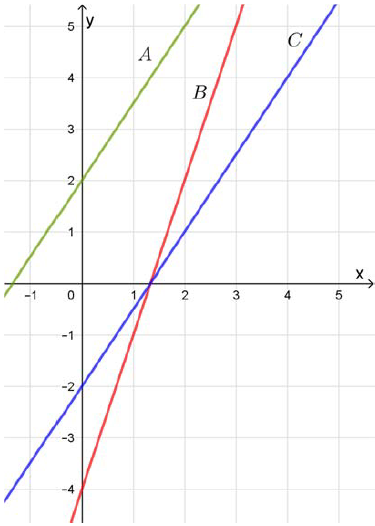
\includegraphics[width=8cm]{Opgave_31-40/Opgave_32/32.png}

Afgør hvilken graf der hører til hvilken funktion. Begrund svaret.

\ans

For en hver lineær funktion gælder det at dens b værdi er skæringen med y aksen.
Da en lineær funktion har den generelle forskrift $f(x) = ax + b$ kan vi altså se at b værdien for de
3 funktioner $f(x), g(x), h(x)$ har forskellige b værdier og dermed forskellige skæringer med y aksen.

Da $f(x)$ har b værdien $b = -4$ skærer den y aksen i $y = -4$ og svarer derfor til den røde lineære funktion B.

Da $g(x)$ har b værdien $b = -2$ skærer den y aksen i $y = -2$ og svarer derfor til den blå lineære funktion C.

Da $h(x)$ har b værdien $b = 2$ skærer den y aksen i $y = 2$ og svarer derfor til den grønne lineære funktion A.